\chapter{绪论}


\section{研究背景和意义}
\label{sec:研究背景和意义}

区块链(Blockchain)最初由中本聪(Satoshi Nakamoto)在2008年提出\cite{nakamoto2008bitcoin},被应用在比特币的创造和交易中。区块链是一种分布式数据库,其核心概念是去中心化和安全性,它将数据存储在多个节点上,并使用密码学技术确保其安全性和完整性。区块链的每个区块都包含了前一个区块的信息以及时间戳,形成了一个不可篡改的链式结构,使得所有的交易记录都可以被验证和追溯。这种技术的应用不仅限于加密货币领域,还可以应用于金融服务、供应链管理、物联网、医疗保健等领域。

随着区块链技术的发展,智能合约(Smart Contract)应运而生。智能合约是一种以代码形式编写的协议,类似于现实世界中的“合同”,而智能合约可以在没有第三方参与的情况下执行交易,实现自动化的规则执行。智能合约的概念最早由尼克·萨博(Nick Szabo)提出,随后由以太坊(Ethereum)创始人维塔利克·布特林(Vitalik Buterin)在以太坊平台上得到了广泛的应用。智能合约的出现使得去中心化的应用成为可能,它们可以自动执行协议、管理数字资产、保证交易的安全性和可靠性。

智能合约的出现极大地推动了区块链技术的应用,但是其自动执行以及不可篡改的特性也导致合约的安全性面临着一系列潜在缺陷,这些缺陷可能带来严重的信任风险和财务损失。事实上,自智能合约问世以来,其代码缺陷导致的金融安全事件层出不穷。2016年,基于以太坊区块链的分散自治组织(The DAO)发生了一起严重的智能合约漏洞事件。攻击者利用智能合约的重入漏洞成功发起了一次针对The DAO的攻击,窃取了价值数百万美元的加密货币。此次事件导致以太币价格暴跌,并引发了一场有关区块链安全性的广泛讨论。2017年,基于以太坊的多重签名钱包服务提供商Parity Technologies发生了一起严重的智能合约漏洞事件。由于智能合约中的一个错误操作,攻击者成功冻结了价值数百万美元的加密货币资产,影响了众多加密货币投资者和交易所的资金安全\cite{niyuandong}。2020年,去中心化交易协议UniSwap中发现了一处智能合约漏洞,导致攻击者利用闪电贷功能成功实施了欺诈。攻击者利用该漏洞进行了大规模交易,导致大量加密货币资产流失。2023年3月,金融借贷平台Euler Finance被黑客攻击。相关合约中的一个关键函数缺少清算检查逻辑,因此攻击者无需任何抵押即可转移清算资金,该漏洞被黑客利用后直接导致价值约1.97亿美元的加密货币被盗。\autoref{fig:attacks_events}展示了近年来发生的智能合约安全事件数量及经济损失。

\begin{figure}[htbp]
    \centering
    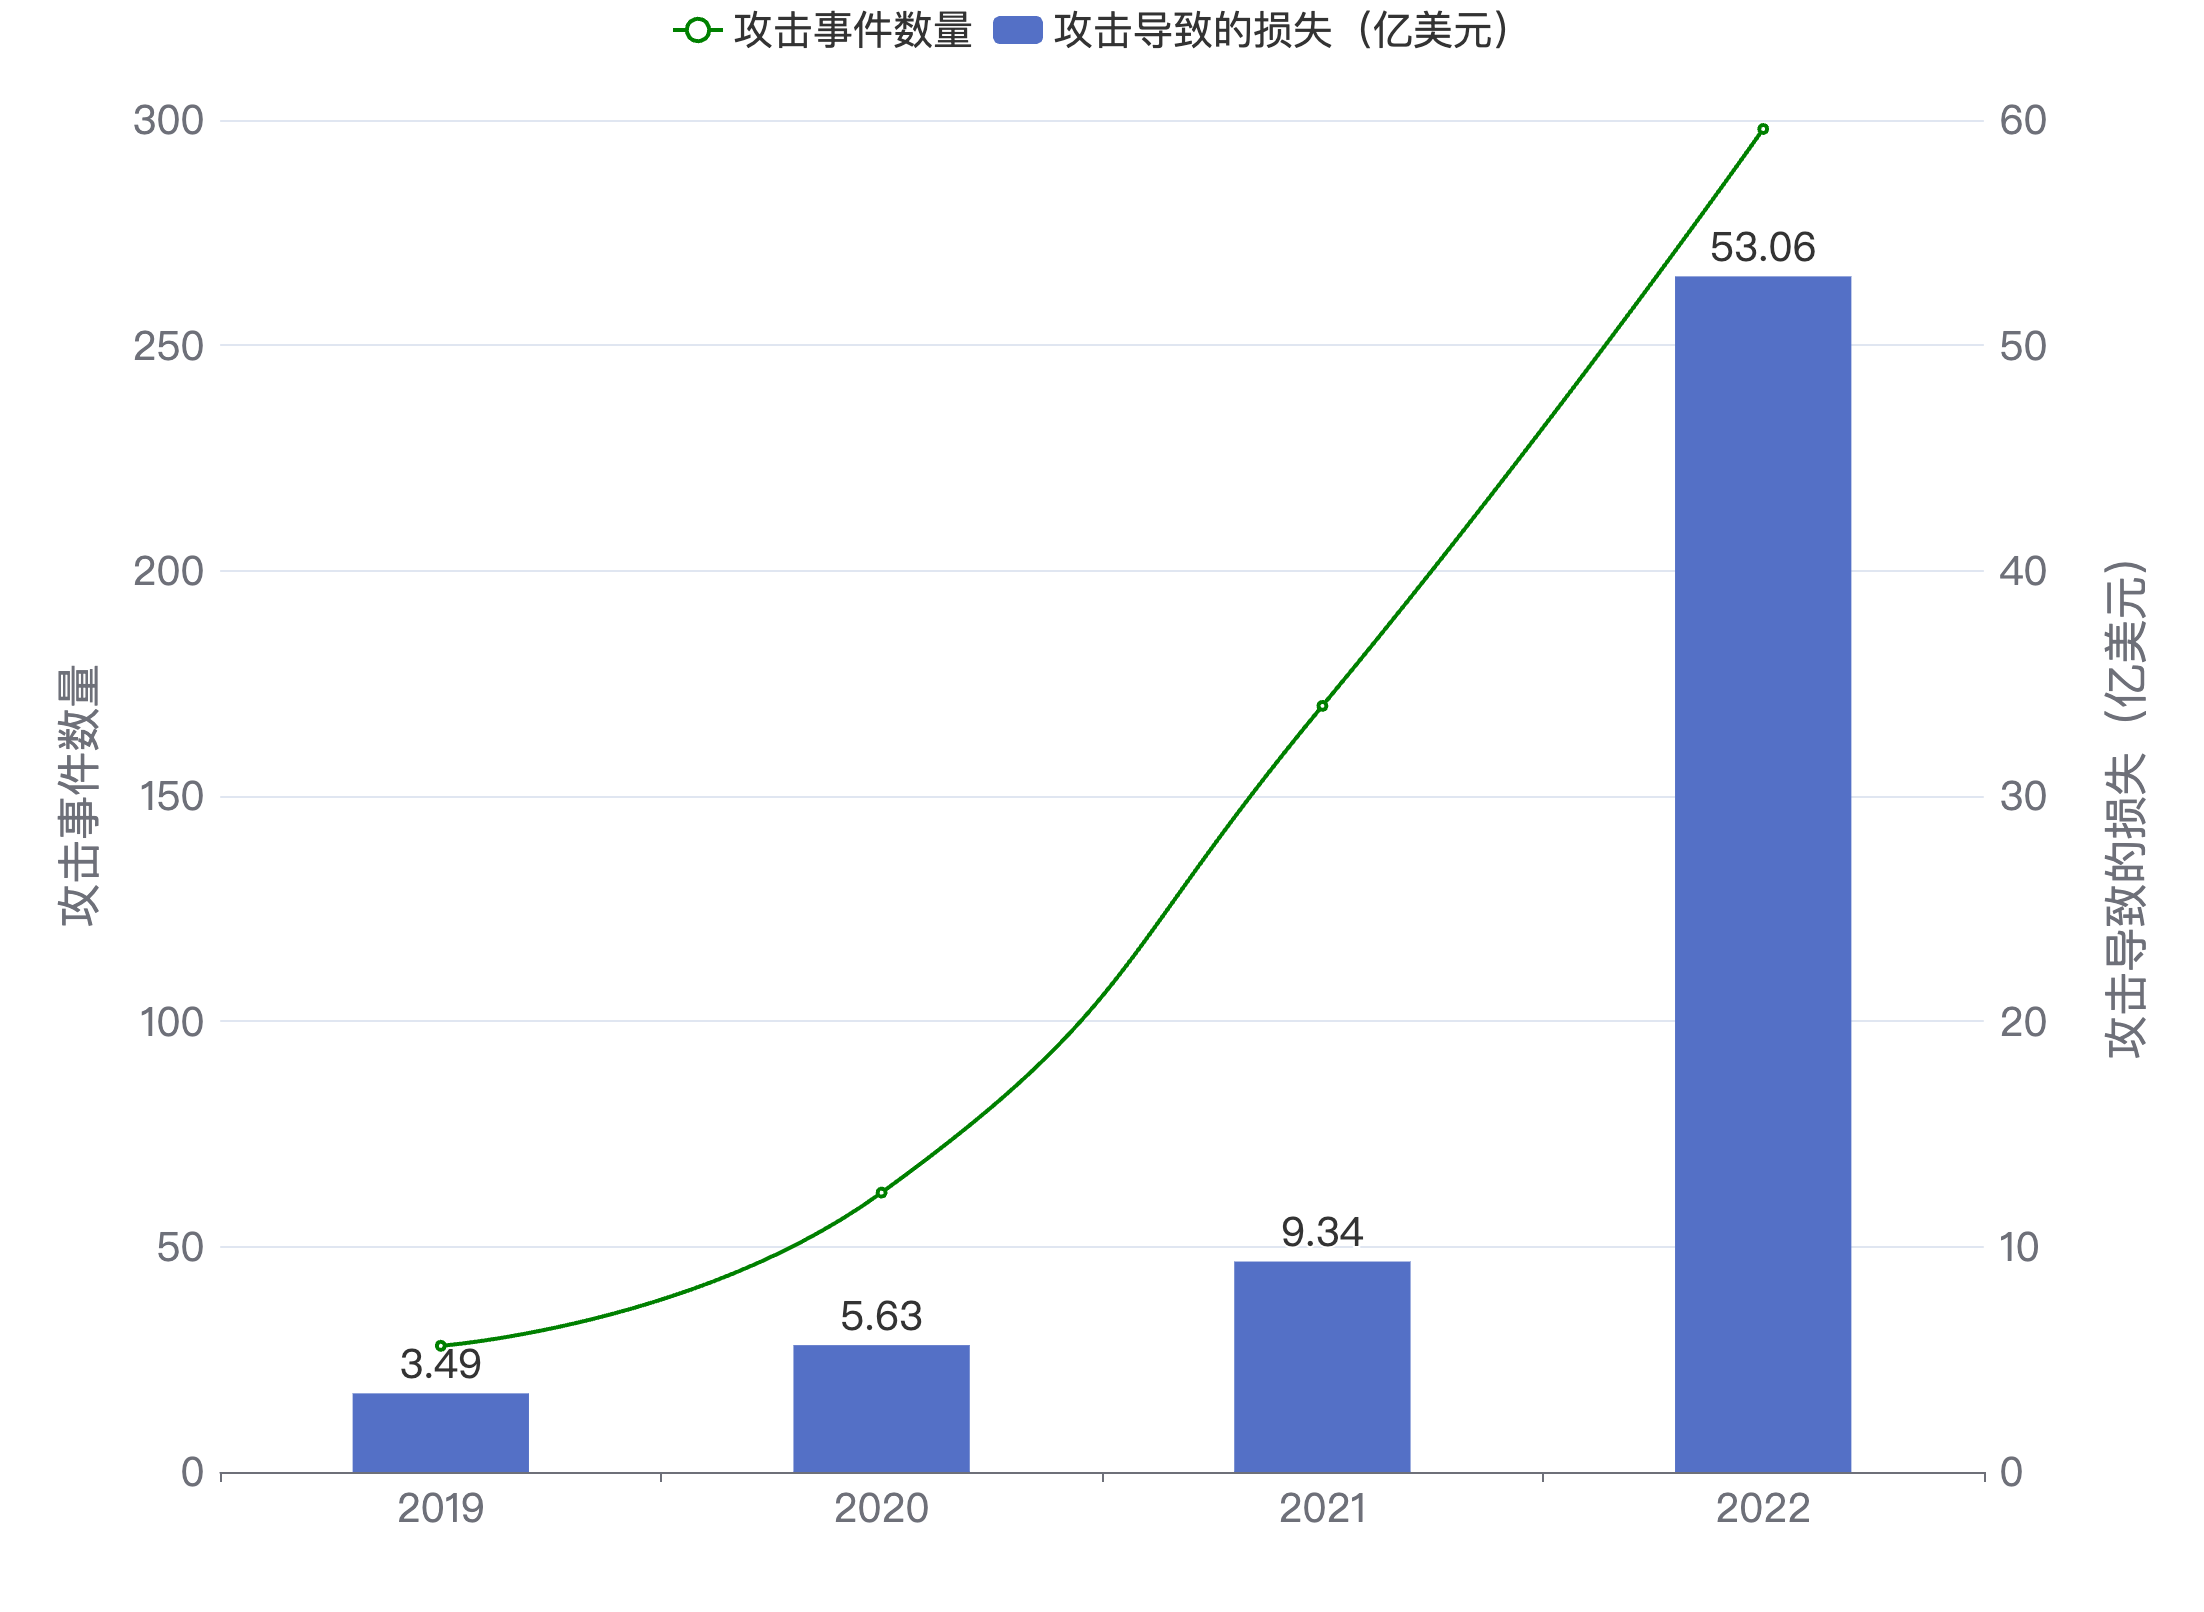
\includegraphics[width=.7\linewidth]{pictures/attacks.png}
    \caption{\label{fig:attacks_events}近年来发生的智能合约安全事件数量及经济损失}
\end{figure}
    
以上事件表明智能合约漏洞严重损害了区块链社区对于智能合约安全性的信任,可能给参与者带来严重的经济损失和信任危机,进一步凸显了智能合约安全性的重要性。为了提高智能合约的安全性,已经诞生了一些专业的第三方机构,如Cyfrin、OpenZeppelin、慢雾科技等。他们会对智能合约代码进行全面的审计和分析,以识别低效代码以及潜在的漏洞,最终出具一份专业的审计报告。开发者可以凭此审计报告声明智能合约的安全性,进而获得区块链社区以及用户的信任,为自己的应用进行担保。然而不幸的是,专业机构通常需要收取高昂的审计费用,这往往让大多数开发者望而却步。因此,利用智能软件工程领域的研究方法对智能合约的质量进行分析是十分必要的。


% 事实上,从智能合约诞生以来,借助软件工程领域的技术对智能合约进行漏洞检测(Vulnerability Detection)的研究从未停止。然而迄今还没有出现一种漏洞检测方法或工具被众多区块链社区采纳,\underline{因此本文对漏洞检测技术的研究是十分必要的}。


\section{国内外研究现状}
\label{sec:国内外研究现状}
针对层出不穷的智能合约安全事件,国内外软件工程领域对智能合约漏洞检测已有相当多的研究工作,接下来本文将介绍多种智能合约漏洞检测方法,以及介绍智能合约运行时崩溃预测的研究现状,为下文本研究的开展奠定基础。
\subsection{智能合约漏洞检测研究现状}
\label{sec:智能合约漏洞检测研究现状}
区块链因其安全性备受关注,然而智能合约中的漏洞所导致的安全问题却在一定程度上制约了区块链应用的流行,这种矛盾吸引了开发者和研究人员对智能合约漏洞检测技术的探索。目前已经诞生了多种漏洞检测方法,主要包括三类:静态分析法、动态分析法和机器学习法。
静态分析法是指在不运行智能合约的前提下进行漏洞检测,主要包括以下方法:形式化验证法、符号执行法、污点分析法;动态分析法则是指在智能合约运行过程中进行漏洞检测,主要指模糊测试法;机器学习法主要包括利用传统的机器学习模型或人工神经网络模型对智能合约进行漏洞检测的方法。
\autoref{tab:defect_detection_methods}中列出了每一种智能合约漏洞检测方法的名称、相关的论文数量及代表方法。

\begin{table}[htbp]
    \caption{\label{tab:defect_detection_methods}现有的智能合约漏洞检测论文数量及代表方法}
    \small
    \begin{threeparttable}
        {
            \renewcommand{\arraystretch}{1.5}
        \begin{tabularx}{\linewidth}{cp{3cm}<{\centering}p{3cm}<{\centering}X<{\centering}}
            \toprule
            类别                     & 方法名称   & 相关论文数量* & 代表方法 \\ \midrule
            \multirow{3}{*}{静态分析法} & 形式化验证法 & 15    & ZEUS\cite{kalra2018zeus}、VaaS\cite{garfatta2021survey}  \\
                                   & 符号执行法  & 9    & Oyente\cite{luu2016making}、TeEther\cite{krupp2018teether}  \\
                                   & 污点分析法  & 8    & Mythril\cite{mythril}、Sereum\cite{rodler2018sereum}  \\ \midrule
            动态分析法                  & 模糊测试法  & 16    & ContractFuzzer\cite{jiang2018contractfuzzer}、Reguard\cite{liu2018reguard}、ILF\cite{he2019learning}  \\ \midrule
            \multirow{2}{*}{机器学习法} & 传统机器学习法  & 32    & Soliaudit\cite{liao2019soliaudit}、Dynamit\cite{Dynamit}、TMLVD\cite{TMLVD}  \\
                                   & 深度学习法  & 25    & SaferSC\cite{tann2018towards}、DR-GCN\cite{zhuang2021smart}、AME\cite{liu2021smart}  \\ \bottomrule
        \end{tabularx}
        }
        \begin{tablenotes}
            \footnotesize
            \item[*] 每种方法相关的论文数量统计范围为2015年至2023年
        \end{tablenotes}
    \end{threeparttable}
\end{table}

\subsubsection{形式化验证法}
    
    形式化验证法利用数学语言和逻辑表达式,将智能合约中的逻辑关系转换为形式规范,通过数学推理和证明,发现可能存在的逻辑错误、漏洞和不安全的设计,从而提前识别潜在的风险。然而,形式化验证法也面临一些挑战,比如对于复杂合约的处理可能较为繁琐,且需要深厚的数学和形式化知识。
    
    2018年,Grishchenko等人首次提出了以太坊虚拟机字节码的小步骤语义\cite{grishchenko2018semantic}(Small-Step Semantics),对合约源代码利用F*框架进行形式化得到可执行代码,并成功在以太坊官方测试套件中验证通过。
    同年,Hildenbrandt等人提出了KEVM框架\cite{hildenbrandt2018kevm},它可以基于K框架对智能合约的部分语义进行形式化分析,以检测出合约中的错误和漏洞。
    Amani等人提出了基于Isabelle方法改进而来的Isabelle/HOL方法\cite{amani2018},它先对智能合约进行EVM字节码级别的逻辑扩展,然后借助F框架生成形式化模型,以此验证代码逻辑中可能存在的问题。
    Kalra等人提出的ZEUS工具\cite{kalra2018zeus}首先将高级语言编写的智能合约转换为中间表示(Intermediate Representation),然后利用抽象解释、符号模型检查和约束语句等形式化方法来检验其安全性。他们构建的原型工具在以太坊平台上评估了超过22.4k个智能合约,结果表明约94.6\%受检验的合约包含潜在漏洞。
    2019年,成都链安科技推出了一个面向EVM的形式化验证平台Vaas\cite{lianan},它可以对智能合约进行10大类32小项的安全检测和验证,准确定位风险代码并提出修改建议。

    \subsubsection{符号执行法}
    
    符号执行法将合约中的变量和输入符号化,用符号代替实际数值,合约的执行路径就不再依赖于具体的输入,研究人员就可以基于符号值进行推演,这使得符号执行法能够遍历多个可能的执行路径。同时,通过对符号值的范围进行分析,可以发现一些算术异常或者条件不当的分支等问题。然而,符号执行法也面临路径爆炸和对合约复杂性的适应性等问题。
    
    2016年,Luu等人提出了一个名为Oyente\cite{luu2016making}的符号执行工具,它首先针对EVM字节码构建控制流图,然后基于控制流图进行符号执行以得到合约的执行路径信息,对之进行分析从而检测出潜在的漏洞,支持检测重入漏洞、异常处理漏洞、交易顺序依赖漏洞。随后的许多工作对Oyente进行了扩展,例如Nikolic等人提出的Maian\cite{maian}进一步扩展了检测的漏洞类型,增加了不定资产冻结、资产泄漏和合约自毁等类型。
    2018年,以太坊官方发布了一个名为Mythril\cite{mythril}的智能合约漏洞检测工具。Mythril使用符号执行法来探索所有可能的不安全路径,能检测出14种智能合约漏洞,如时间戳依赖、任意地址写入和整数溢出。
    同年,还有一批智能合约漏洞检测工具被提出来。Securify\cite{tsankov2018securify}是一种自动化且可扩展的以太坊智能合约漏洞检测工具,利用符号执行法分析合约的依赖图,从中提取语义信息并检验是否存在不安全的模式,通过定义领域相关的不安全模式可以实现扩展性。
    Krupp等人制定了一个缺陷合约的通用定义,并以此构建了TeEther\cite{krupp2018teether}工具,它可以对EVM字节码进行分析是否符号缺陷合约的定义。Sereum\cite{rodler2018sereum}则主要是对EVM在运行时进行监视,根据其运行状态来检测合约的重入漏洞。
    \subsubsection{污点分析法}
    
    污点分析法将合约中的敏感数据视为“污点”,如转账金额、用户身份信息、用户输入,并追踪这些敏感数据在合约内的函数调用或变量操作,从而揭示潜在的漏洞和风险\cite{tongjunchen}。然而,在面临复杂的数据流和动态调用的合约逻辑时,该方法识别出潜在漏洞的能力也会下降。
    
    2018年,Torres等人提出了结合污点分析和符号执行的智能合约安全分析框架Osiris\cite{torres2018osiris}。该框架利用符号执行法对EVM字节码构建控制流图,分析和跟踪污点的传播路径,可以精确检测出合约中的整数漏洞。
    2019年,Gao等人提出了一个名为Easyflow\cite{gao2019easyflow}的智能合约安全分析框架,主要针对溢出漏洞。该框架工作在EVM运行时,在合约的运行过程中对污点进行分析跟踪,实现检测智能合约漏洞的目的。
    \subsubsection{模糊测试法}
    
    模糊测试法会生成大量具有随机性的输入数据,模拟各种可能的用户输入,包括超出正常范围的数值、或者其他可能导致合约异常行为的情况,从而发现智能合约可能存在的安全漏洞。然而,这种方法也有一些局限性,比如需要大量的测试用例、难以涵盖所有可能的输入情况以及可能产生大量误报的问题。
    
    2018年,Jiang等人提出了一个名为ContractFuzzer\cite{jiang2018contractfuzzer}的智能合约检测工具。它采用模糊测试方法生成大量输入,同时借助EVM日志工具记录合约在运行时的行为日志,然后分析这些日志以发现缺陷。
    同年,Liu等人提出的ReGuard\cite{reguard}主要针对智能合约中潜在的重入漏洞。ReGuard通过模糊测试生成随机且多样化的测试数据,并在合约运行时进行监控以实现对重入漏洞的动态识别。但是它将Solidity语言编写的智能合约转换为C++语言,并基于有限状态机模型生成交易以检测缺陷。然而,Solidity语言和C++语言是两种不同的语言。转换后不可避免地会导致部分语法和语义信息的丢失。
    2020年,Torres等人提出了ConFuzzius\cite{confuzzius}漏洞检测工具,首先对合约进行模糊测试以检测简单的漏洞,然后通过符号执行和约束求解生成满足复杂条件的输入,从而对合约的复杂逻辑进行检验。
    2021年,Choi等人开源了一个实用的检测工具SMARTIAN\cite{smartian}。它通过对智能合约字节码的静态分析来预测交易顺序,并决定每个交易是否应满足某些约束。在模糊测试阶段,该工具利用先前的信息构建初始种子语料库,并执行动态数据流分析,根据数据流有效地引导模糊测试。

    
    \subsubsection{机器学习法}
    
    机器学习方法的核心思想是通过手工或者自动提取智能合约的各种漏洞特征,并训练机器学习模型或深度学习模型,最后对新的合约进行漏洞预测。机器学习法可以从包含已知漏洞的数据样本中学习到智能合约的关键特征,从而在新的合约中识别潜在的安全问题。特别是深度学习模型,如循环神经网络(RNN)或长短时记忆网络(LSTM),能够更好地应对合约中复杂的逻辑和数据流。相比于前文提到的传统方法,机器学习法为智能合约漏洞检测提供了一种创新的、高效的解决方案\cite{cui2024}。

    2018年,Tann等人提出的SaferSC\cite{tann2018towards}主要利用长短时记忆网络(Long short-term memory, LSTM)快速检测智能合约漏洞,这也是首次深度学习方法和智能合约漏洞检测相结合。随着合约的复杂度增加,SaferSc保持几乎恒定的分析时间,此外还能发现符号执行工具误报漏洞的合约。

    2020年,Zhuang等人提出了一种名为DR-GCN\cite{zhuang2021smart}的智能合约检测方法,它可以检测以太坊和Viterbi链上多种智能合约漏洞,通过图神经网络实现。首先构建图表示的智能合约函数的语法和语义结构,再利用无量纲图卷积神经网络检测智能合约漏洞。
    % DR-GCN作为基于图神经网络的漏洞检测模型,比较擅长在直接在图形数据上学习表示并理解其中的复杂关系,实验结果表明该方法能够有效检测出三种智能合约漏洞:重入漏洞、时间戳依赖漏洞、无限循环漏洞。

    \begin{figure}[htbp]
        \centering
        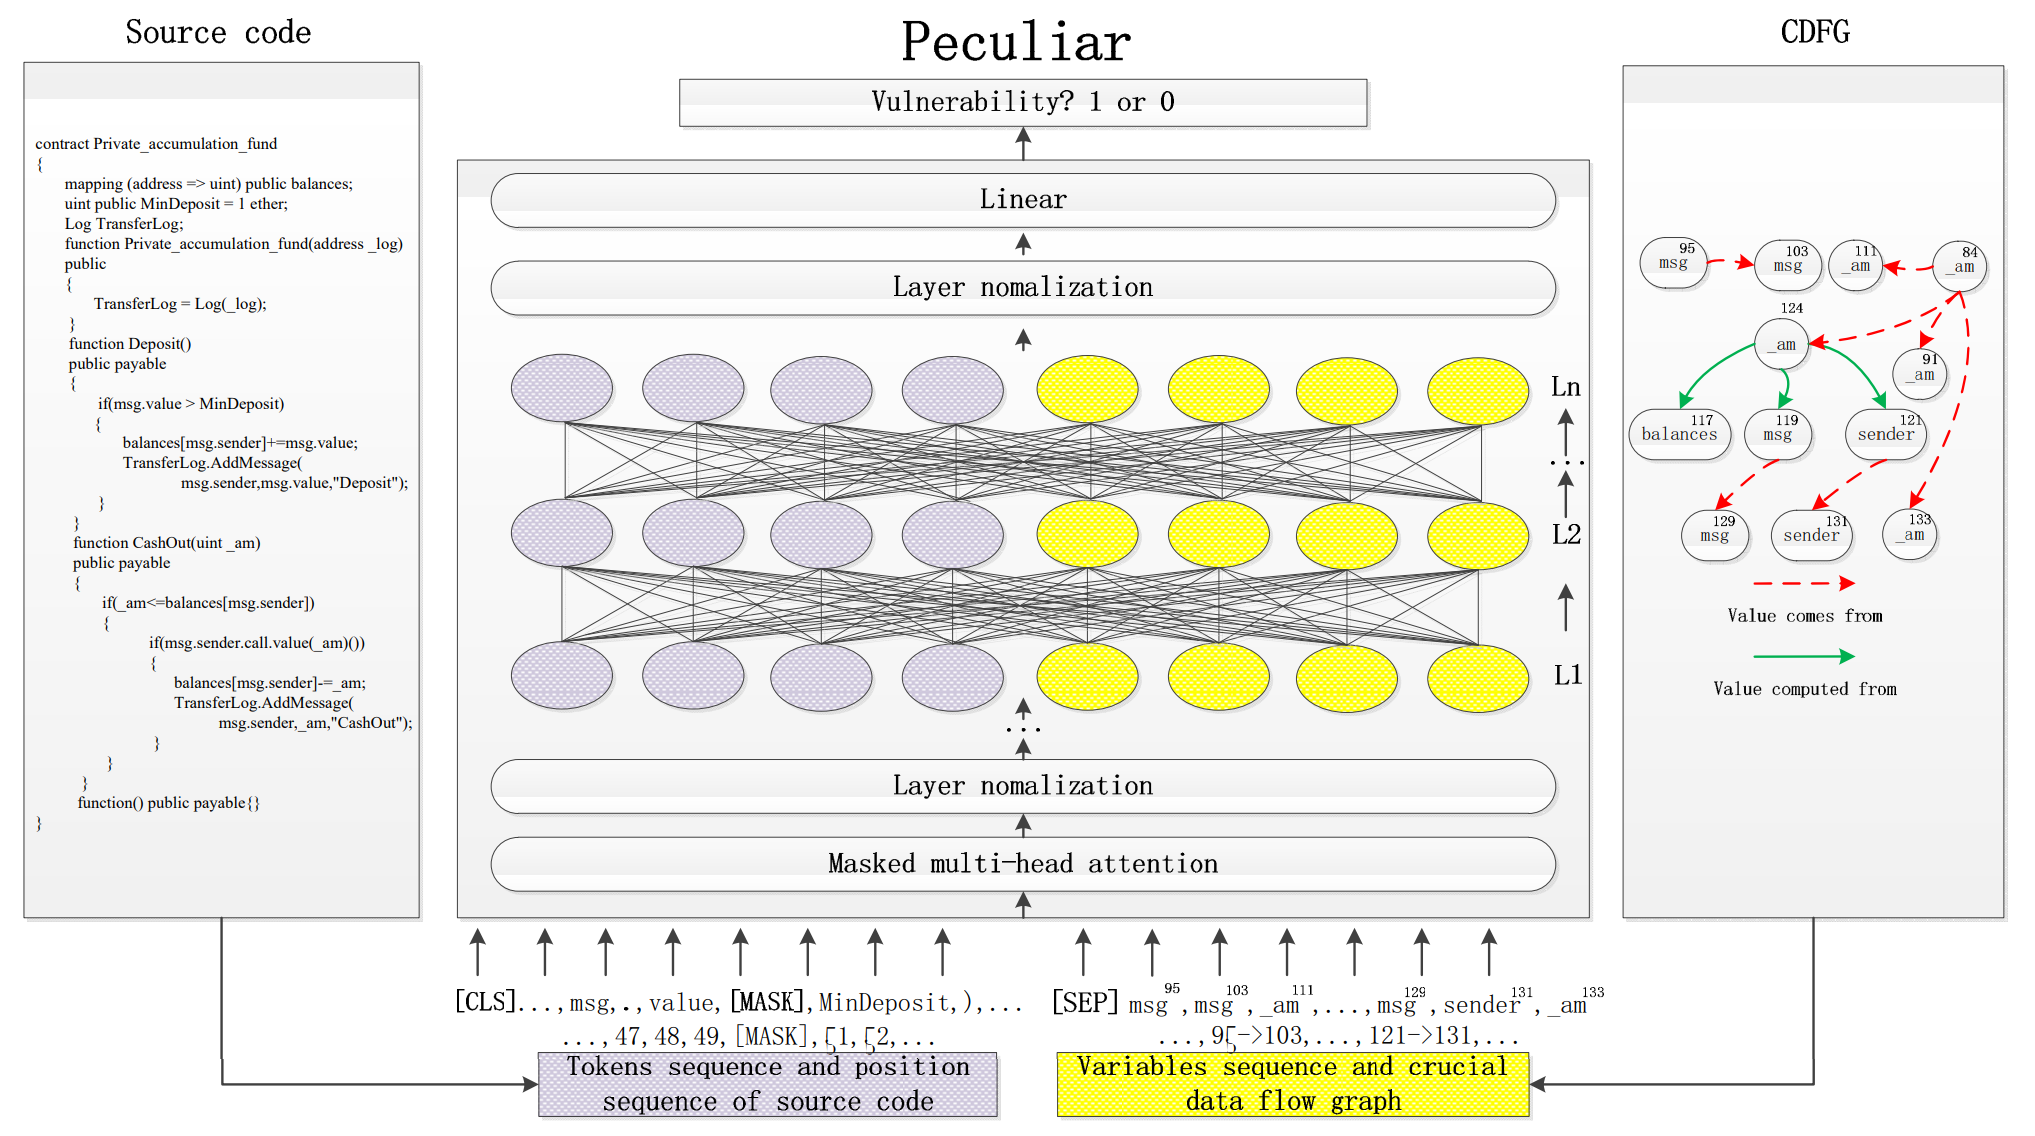
\includegraphics[width=\linewidth]{pictures/peculiar}
        \caption{\label{fig:peculiar}Peculiar方法的框架图}
    \end{figure}
    
    2021年,Liu等人提出的AME\cite{liu2021smart}模型结合了深度学习和专家模式。从源代码中提取的专家模式包含合约的局部信息,同时利用图结构来构建合约的控制流和数据流语义,最后使用注意力多编码器网络融合专家模式和语义图进行漏洞预测。实验证明该方法显著优于原先基于静态或动态分析的方法。

    同年,Wu等人提出的Peculiar方法\cite{wu2021peculiar}首次将预训练模型应用到智能合约漏洞检测任务中,他们从智能合约源代码中提取了数据流图,并根据重入漏洞的特点将数据流图进行精简,得到关键数据流图(Crucial Data Flow Graph, CDFG),实验结果表明该方法在检测重入漏洞时可以达到91.8\%的精确率和92.4\%的召回率,显著优于当时的最优方法Smartcheck\cite{smartcheck},同时消融实验表明,关键数据流图和预训练模型的应用在该方法中发挥了重要作用。\autoref{fig:peculiar}显示了Peculiar方法的框架图。受此启发,本文也将数据流图和预训练模型应用到智能合约漏洞检测和运行时崩溃预测任务中。
    

% \textcolor{red}{这里可能需要扩充,说明每种方法的应用情况,对比不同方法}


\subsection{智能合约运行时崩溃研究现状}
\label{sec:智能合约运行时崩溃研究现状}
通过在各大文献数据库中搜索,关于智能合约运行时崩溃的研究工作寥寥无几,只有一些工作对以太坊虚拟机的执行过程中出现的异常进行了研究。


2020年,Wang等人提出了一个名为ExecuWatch\cite{wang2020onthe}的原型工具,首先对智能合约进行静态分析推断需要记录执行状态的位置,并对其注入日志语句以打印调试信息,然后使用模糊测试法在100多个智能合约的326个公共函数上进行测试。日志中记录了所有合约的执行细节,通过分析这些日志便可以定位到失败合约中的异常语句。
同年,Jumnongsaksub等人\cite{reducing2020}对如何减少以太坊上智能合约的执行异常进行了探究,提出了Evitar算法用于动态分析已完成的交易,并在用户提交新的交易之前就潜在错误发出警告,实验结果显示,借助Evitar算法的智能合约运行时异常减少了79\%,消耗的Gas总量减少了73\%。
2021年,Oliviera等人\cite{oliveira_analyzing_2021}从多个来源\footnote{https://www.etherscan.io}\footnote{https://www.etherchain.com}收集了超过200万个以太坊交易数据,其中有一小部分是执行失败的交易。他们对数据集进行了平衡处理,并使用随机森林、逻辑回归、支持向量机等机器学习模型进行训练预测交易的执行结果,结果表明随机森林在ROC和F1-score指标上具有最好的效果,同时分析了交易成功与否的原因主要取决于网络的拥塞情况和用户提供的Gas多少。

2023年,Yu等人提出了名为TxMirror的分析工具\cite{Yu_2023},他们使用爬虫连接以太坊获取交易信息,并在本地运行一个以太坊虚拟机模拟交易,当数据发生变化或执行某些操作码时,分析器会根据设定的异常规则匹配数据信息,当发现攻击或漏洞时将其写入报告中。
同年,Ivanov等人设计了一个交易测试工具TxT\cite{IvanovTxT}。用户首先将其加密钱包连接到TxT网络,然后提交新的交易,Txt框架会模拟交易,持续检查测试交易在区块链当前状态下是否具有相同的执行路径,用户在交易完成后观察交易结果(如加密货币余额、代币余额、错误信息等)是否符合预期。如果测试执行的结果符合预期,用户便可以将钱包切换回以太坊主网,并像往常一样提交交易。结果表明,Txt能识别大多数与已知漏洞相关的交易,并具有较高的覆盖率。

% \textcolor{red}{这里需要扩充一下,说明虽然静态和动态分析法已经有非常多的研究工作,也有广为人知的工具。但是在某些方面还是存在劣势,而机器学习法正好能够弥补这些不足,所以探究更高效的机器学习法是十分必要且有意义的。
% 随着被部署在以太坊上的智能合约数量呈爆 炸 性 增 长 ,
% 对合约中的潜在漏洞进行更加准确而更高效的检查变得愈发
% 重要 . 而上文提到的传统自动漏洞检测工具都需要大量的计
% 算开销 , 有时甚至需要探索所有路径或是到达一定深度才能
% 够检测到漏洞 , 非常耗时且检测效率不高 . 而基于机 器 学 习
% 的检测方法通过对不同形式的合约代码进行自动化的特征提
% 取和恰当的模型训练 , 显著提高了检测效率 , 使其具有更好的
% 泛化能力 , 适用于更多的应用场景 , 并且相比现有工具在一定
% 程度上提高了对常见漏洞的检测准确率 .
% }

\section{本文的研究内容}
\label{sec:本文的研究内容}
% 在区块链技术不断发展的今天,智能合约的安全性成为了研究的重点。尽管静态和动态分析技术已经得到广泛应用,并催生出许多知名的工具,但它们在某些方面仍有局限性。深度学习作为一种新兴的方法,正逐步展现出其在弥补传统技术不足方面的巨大潜力。因此,深入研究和优化基于深度学习的智能合约漏洞检测方法显得尤为关键和有价值。

随着智能合约在以太坊等平台上的迅猛增长,准确且高效地识别潜在的安全漏洞变得更加紧迫。传统的自动漏洞检测工具往往需要大量的计算资源,有时甚至需要遍历所有可能的执行路径或达到一定的分析深度,这不仅耗时而且效率不佳。相对而言,基于深度学习的方法通过自动化提取合约代码的多样特征,并结合精确的模型训练,不仅显著提升了检测的效率,而且增强了方法的泛化能力,使其适用于更广泛的场景。此外,这种方法在提高对常见漏洞检测的准确率方面也表现出色,相比现有的工具有着明显的优势。本文正是在这个背景下,基于深度学习预训练模型,提出了一种融合静态代码指标和语义特征进行智能合约漏洞检测的方法。本文的研究内容如下:
\begin{enumerate}[label=(\arabic*)]
    \item 基于静态代码指标和语义特征融合的智能合约表征。
    
    静态代码指标在软件工程研究领域起着至关重要的作用,不仅能够反映代码的结构特性,还易于获取。本文将探究一些契合智能合约源代码的静态代码指标,并尝试利用相关工具提取这些指标,用于表示智能合约的结构特征。同时,抽象语法树作为源代码编译时的中间产物,保留了全面且丰富的程序语义信息,但其本身过于复杂的层次结构难以直接进行研究,因此本文将尝试从其中提取关键语义图用于表达智能合约的语义信息。然后,本文将在上述基础上尝试融合这两种特征,用于表征智能合约的结构特征和语义信息,以便于开展下一步研究。
    \item 基于深度学习的智能合约漏洞检测研究。
    
    深度学习在智能合约漏洞检测方面表现出色,但是只有良好的合约表征与合适的深度学习模型才能取得出色的效果。因此本文将在上一步研究的基础上,使用深度学习法对智能合约的静态代码指标和语义图进行嵌入,以生成其在高维空间的向量表示,然后以此作为输入训练智能合约的漏洞检测模型。另一方面,预训练模型通过大规模文本数据进行训练,学习了丰富的文本表示形式,在深度学习领域得到了广泛应用,本文将尝试探索CodeBERT类似的代码领域预训练模型,并将其作为基础模型结合上一步得到的智能合约表征,探究智能合约的漏洞检测方法。
    \item 基于深度学习的智能合约运行时崩溃预测研究。
    
    针对目前智能合约运行时崩溃导致交易失败的相关研究较少的情况,本文欲在上一步工作的基础上,丰富智能合约数据集中交易结果相关的信息,并利用特征融合的漏洞检测模型对智能合约运行结果进行预测,开展实验并分析结果,探究智能合约各种漏洞与运行时崩溃之间的关系。
    
\end{enumerate}
\section{本文的组织结构}
\label{sec:本文的组织结构}
第一章:绪论。本章首先阐述了智能合约漏洞检测工作的研究背景和意义,分析了现有工作提出的方法和存在的问题,紧接着介绍了该领域在国内外的研究现状,引出了智能合约在运行时崩溃的研究问题,最后介绍了本文的主要研究内容和组织架构。


第二章:相关理论和技术。本章首先介绍了以太坊中的一些关键特性,如账户、交易、Gas机制等,然后介绍了智能合约的概念和常见的漏洞类型,以及智能合约运行崩溃原因。接着介绍了静态代码指标和语义特征的含义,包括特征融合技术及其在软件工程领域的应用情况。最后介绍了预训练模型以及代码领域预训练模型的相关概念,包括其在漏洞检测工作中的应用情况。

第三章:基于特征融合的智能合约漏洞检测方法。本章是本文的核心章节之一。首先定义了34个智能合约中的静态代码指标,然后引入了三种智能合约语义图用于提取语义特征,并介绍了提取语义特征的方法。下一部分介绍了数据集的搜集、预处理与标注工作。然后着重介绍了本文提出的方法的核心:基于特征融合的漏洞检测模型,包括模型架构、预训练任务、特征融合等。最后介绍了实验设计,包括实验环境、参数设置、评估指标等,并对实验结果进行了详细分析。

第四章:智能合约运行时崩溃的预测方法探究。本章首先介绍了该研究的背景和动机,然后介绍了在上一步研究的基础上对数据集的改进,设计了研究方法,最后描述了实验方案并对实验结果进行了深入的分析。

第五章:总结与展望。作为本文的最后一章,本章主要包含两部分内容,第一部分对全文进行总结并对本文的主要贡献进行了梳理;第二部分对本文存在的不足之处进行了剖析,并提出了改进的方向。

% \section{本章小结}
% \label{sec:本章小结1}
% 本章首先简单介绍了区块链技术和智能合约的发展历程,以及智能合约漏洞可能导致的风险,以现实世界的实例说明了智能合约中的漏洞造成的经济损失和信任危机。然后对
